%%%%%%%%%%%%%%%%%%%%%%%%%%%%%%%%%%%%%%%%%%%%%%%%%%%%%%%%%%%%%%%%%%%%%%
% LaTeX Example: Project Report
%
% Source: http://www.howtotex.com
%
% Feel free to distribute this example, but please keep the referral
% to howtotex.com
% Date: March 2011 
% 
%%%%%%%%%%%%%%%%%%%%%%%%%%%%%%%%%%%%%%%%%%%%%%%%%%%%%%%%%%%%%%%%%%%%%%
% How to use writeLaTeX: 
%
% You edit the source code here on the left, and the preview on the
% right shows you the result within a few seconds.
%
% Bookmark this page and share the URL with your co-authors. They can
% edit at the same time!
%
% You can upload figures, bibliographies, custom classes and
% styles using the files menu.
%
% If you're new to LaTeX, the wikibook is a great place to start:
% http://en.wikibooks.org/wiki/LaTeX
%
%%%%%%%%%%%%%%%%%%%%%%%%%%%%%%%%%%%%%%%%%%%%%%%%%%%%%%%%%%%%%%%%%%%%%%
% Edit the title below to update the display in My Documents
%\title{Project Report}
%
%%% Preamble
\documentclass[paper=a4, fontsize=11pt]{scrartcl}
\usepackage[T1]{fontenc}
\usepackage{fourier}

\usepackage[protrusion=true,expansion=true]{microtype}	
\usepackage{amsmath,amsfonts,amsthm} % Math packages
\usepackage[pdftex]{graphicx}	
\usepackage{url}
\usepackage[brazil]{babel}
\usepackage[utf8]{inputenc}
\usepackage[T1]{fontenc}
\usepackage{graphicx}
\usepackage{subcaption}
\usepackage{multicol}

%%% Custom sectioning
\usepackage{sectsty}
\allsectionsfont{\centering \normalfont\scshape}


%%% Custom headers/footers (fancyhdr package)
\usepackage{fancyhdr}
\pagestyle{fancyplain}
\fancyhead{}											% No page header
\fancyfoot[L]{}											% Empty 
\fancyfoot[C]{}											% Empty
\fancyfoot[R]{\thepage}									% Pagenumbering
\renewcommand{\headrulewidth}{0pt}			% Remove header underlines
\renewcommand{\footrulewidth}{0pt}				% Remove footer underlines
\setlength{\headheight}{13.6pt}


%%% Equation and float numbering
\numberwithin{equation}{section}		% Equationnumbering: section.eq#
\numberwithin{figure}{section}			% Figurenumbering: section.fig#
\numberwithin{table}{section}				% Tablenumbering: section.tab#


%%% Maketitle metadata
\newcommand{\horrule}[1]{\rule{\linewidth}{#1}} 	% Horizontal rule

\title{
	%\vspace{-1in} 	
	\usefont{OT1}{bch}{b}{n}
	\normalfont \normalsize \textsc{Universidade Federal do Ceará} \\ [25pt]
	\horrule{0.5pt} \\[0.4cm]
	\huge Reconhecimento de Padrões \\
	\horrule{2pt} \\[0.5cm]
}
\author{
	\normalfont 								\normalsize
	João Rafael Barbosa de Araujo\\[-3pt]		\normalsize
	\today
}
\date{}


%%% Begin document
\begin{document}
	\maketitle
	
	Esse relatório contém as respostas para o segundo trabalho da disciplina de Reconhecimento de padrões. Além de um curto resumo das diferentes técnicas de validação e classificação utilizados no trabalho, assim como os resultados das diferentes técnicas aplicadas ao banco de dados \textit{iris\_log} e \textit{dermatology} de acordo com o que foi solicitado nas questões.
	
	\newpage
	
	\section{Primeira questão}
	
	\textbf{Usando o conjunto de dados do aerogerador (variável de entrada: velocidade do vento – m/s, variável de saída: potência gerada – kWatts), determine o modelo de regressão polinomial (graus 2, 3, 4, 5 e 6) com parâmetros estimados pelo método dos mínimos quadrados.}
	
	
	\textbf{ Avaliar a qualidade de cada modelo por meio do coeficiente de determinação (R²). }\\
	
	Regressão polinomial é uma regressão feita a partir de combinações não lineares das entradas. Essa regressão é utilizada para tentar representar dados que não são linearmente comportados, em que é estendido o conceito de regressão linear a partir da criação de novas variáveis polinomiais a partir de combinações das entradas originais.
	
	Na Figura \ref{fig:fig1} podemos observar que para esse conjunto de dados, aumentar o grau do polinômio resulta em uma melhor aproximação do comportamento dos pontos. Para avaliar a qualidade dessa regressão é utilizado o coeficiente de determinação R². Porém R² não reflete bem a qualidade da regressão, por essa razão alguns autores preferem utilizar R² ajustado onde há uma penalização pelo acréscimo de novas variáveis, podendo assim definir um balanço entre qualidade do regerssor e tamanho do vetor de variáveis de regressão.
	
	Podemos observar que para os graus 2, 3 e 4 o valor de R² subiu a cada novo grau, já no quinto grau vemos que o valor de R² ajustado diminuiu. Quando há a diminuição do valor de R² ajustado é sinal que o grau anterior é o ideal para esse conjunto de dados e que adicionar mais variáveis não vai melhorar significativamente o regressor.
	
	O código utilizado para gerar os resultados pode ser encontrado em \textit{rp\_regressao\_q1.py}.
	
	\newpage
	
	\begin{figure}[h!]
		\begin{subfigure}{.5\textwidth}
			\centering
			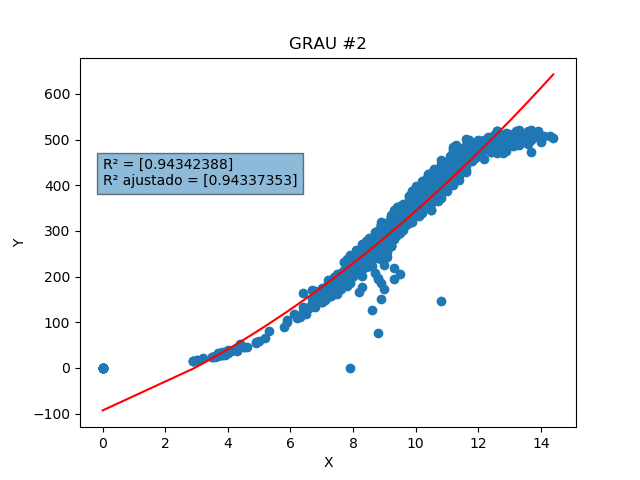
\includegraphics[width=\linewidth]{img/q1_fig_GRAU2.png}
			\caption{Regressão polinomial de grau 2}
			\label{fig:q1grau2}
		\end{subfigure}%
		\begin{subfigure}{.5\textwidth}
			\centering
			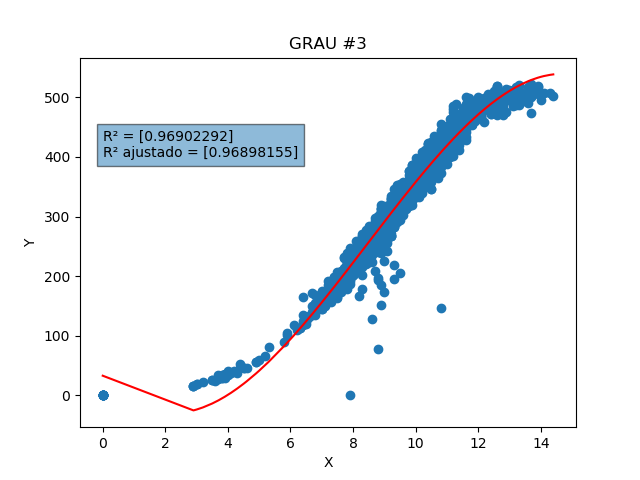
\includegraphics[width=\linewidth]{img/q1_fig_GRAU3.png}
			\caption{Regressão polinomial de grau 3}
			\label{fig:q1_grau3}
		\end{subfigure}
		\begin{subfigure}{.5\textwidth}
			\centering
			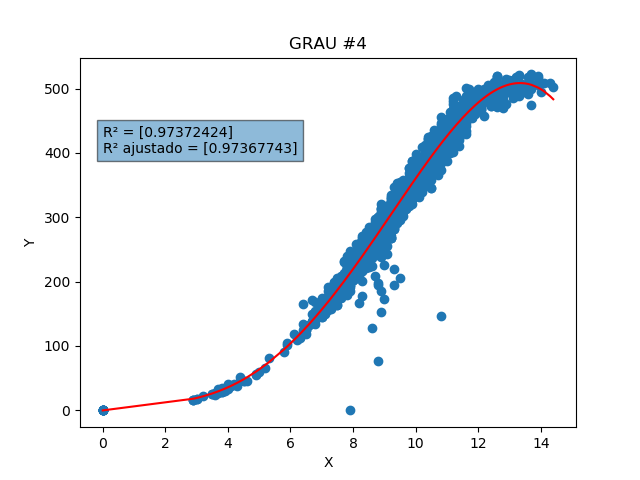
\includegraphics[width=\linewidth]{img/q1_fig_GRAU4.png}
			\caption{Regressão polinomial de grau 4}
			\label{fig:q1grau4}
		\end{subfigure}%
		\begin{subfigure}{.5\textwidth}
			\centering
			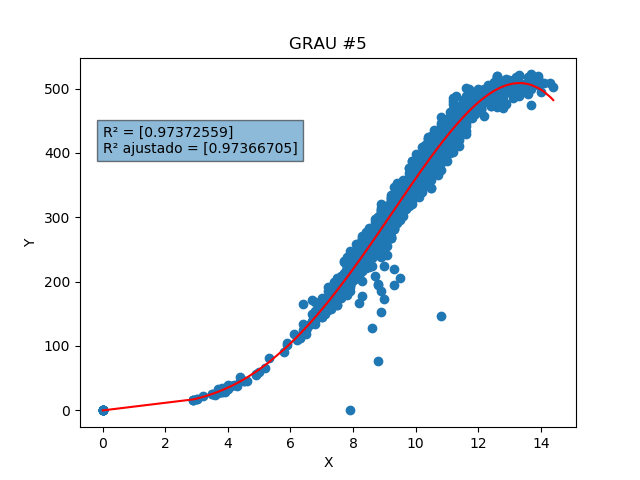
\includegraphics[width=\linewidth]{img/q1_fig_GRAU5.png}
			\caption{Regressão polinomial de grau 5}
			\label{fig:q1_grau5}
		\end{subfigure}
		\begin{subfigure}{.5\textwidth}
			\centering
			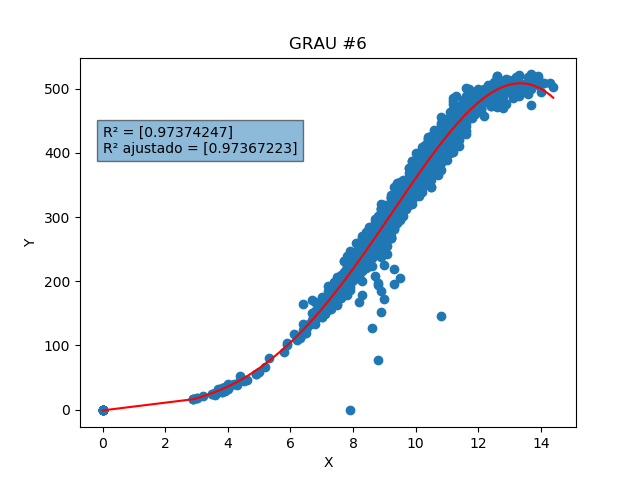
\includegraphics[width=\linewidth]{img/q1_fig_GRAU6.png}
			\caption{Regressão polinomial de grau 6}
			\label{fig:q1grau6}
		\end{subfigure}%
		
		\caption{Regressão polinomial para diferentes graus e respectivos R²}
		\label{fig:fig1}
	\end{figure}
	
	
	\section{Segunda questão}
	
	\textbf{Dada a base de dados abaixo, na qual a primeira e segunda colunas são as variáveis regressoras (x1 e x2) e a terceira coluna é a variável dependente (y), determine o modelo de regressão múltipla (plano) com parâmetros estimados pelo método dos mínimos quadrados. Avalie a qualidade do modelo por meio do coeficiente de determinação (R²).}
	\begin{center}
		
		\textbf{D =[122 139 0.115;\newline
			114 126 0.120;\newline
			086 090 0.105;\newline
			134 144 0.090;\newline
			146 163 0.100;\newline
			107 136 0.120;\newline
			068 061 0.105;\newline
			117 062 0.080;\newline
			071 041 0.100;\newline
			098 120 0.115]; \newline}
	\end{center}
	
	Similar ao que foi feito na questão 1, aqui também iremos calcular diferentes valores de R² ajustado para esse conjunto de dados. Uma diferença para esse bando de dados é que agora temos 2 valores de X para cada amostra.
	\begin{multicols}{2}
    	\begin{verbatim}
    	GRAU = 1
    	R² = [0.72388235]
    	R² ajustado = [-0.1044706]
    	----------------------------
    	GRAU = 2
    	R² = [0.83532045]
    	R² ajustado = [1.6587182]
    	----------------------------
    	GRAU = 3
    	R² = [0.83928699]
    	R² ajustado = [1.21428401]
    	----------------------------
    	GRAU = 4
    	R² = [0.77426695]
    	R² ajustado = [1.18058644]
    	----------------------------
    	GRAU = 5
    	R² = [0.96537463]
    	R² ajustado = [1.01978593]
    	----------------------------
    	GRAU = 6
    	R² = [1.]
    	R² ajustado = [1.]
    	\end{verbatim}
	\end{multicols}
	Para esses dados o valor de R² aumenta até chegar em 1 no sexto grau. 
	Já o comportamento de R² ajustado aumenta inicialmente, e então passa a diminuir a partir do segundo grau. Assim, de acordo com R² ajustado é interessante utilizar até o segundo grau apenas.
	
	O código utilizado para gerar os resultados pode ser encontrado em \textit{rp\_regressao\_q2.py}.
	
	\newpage
	
	\section{Terceira questão}
	
	\textbf{Classificar o conjunto de dados Dermatology disponível em http://archive.ics.uci.edu/ml/datasets.php, conforme as instruções a seguir.}
	\begin{itemize}
		\item \textbf{Classificador: ELM, Perceptron, MLP (implementar os dois primeiros classificadores);}
		\item \textbf{Estratégia de validação cruzada: leave-one-out e 5-fold;}
		\item \textbf{Testar com e sem o zscore;}
		\item \textbf{Montar a matriz de confusão para cada classificação usando os dados de testes. }
	\end{itemize}

	
	
	\subsection{\textbf{Perceptron}}
	Para a implementação do algoritmo de perceptron foi utilizado o livro \textit{Hands-On Machine Learning with Scikit-Learn \& TensorFlow}, onde foi mostrado que existem duas funções de ativação do neuronio que são comumente utilizadas na literatura. Para essa implementação a função utilizada foi \textbf{heaviside()} que retorna 1 para qualquer elemento maior que zero ou retorna zero caso contrário.
	
	Como a rede perceptron tem apenas um neurônio, foi utilizada a técnica \textit{one versus all}, onde a rede foi avaliada para uma classe por vez, ou seja, é testada a capacidade da rede de diferenciar uma classe em relação a todas as outras.
	
	\subsubsection{Leave-one-out}
	
    Como foi falado na introdução dessa seção, os algoritmos de perceptron serão avaliados utilizando \textit{one vs all}. Existem alguns parâmetros de parada que podem ser ajustados dentro do algoritmo da \textit{Perceptron}, dentre eles o numero de atualizações dos peses ou um $\epsilon$ que para a simulação quando o crescimento da aprendizagem se torna muito pequeno.
    
    Para essa simulação foi utilizado o numero de atualizações como critério de parada, esse valor é chamado de \textit{epochs} (do inglês, época).
    
    Abaixo temos a classificação de cada classe de acordo com um certo numero de épocas (sem normalização).
    
	\begin{multicols}{2}
    	\begin{verbatim}
For 4 epochs:
for class:1 Result:98.04 %
for class:2 Result:92.46 %
for class:3 Result:99.72 %
for class:4 Result:94.69 %
for class:5 Result:98.88 %
for class:6 Result:100.00 %
----------------------------
For 5 epochs:
for class:1 Result:97.77 %
for class:2 Result:90.78 %
for class:3 Result:99.44 %
for class:4 Result:94.41 %
for class:5 Result:99.72 %
for class:6 Result:100.00 %
----------------------------
For 6 epochs:
for class:1 Result:98.32 %
for class:2 Result:93.85 %
for class:3 Result:100.00 %
for class:4 Result:94.13 %
for class:5 Result:99.72 %
for class:6 Result:100.00 %
----------------------------
For 7 epochs:
for class:1 Result:98.60 %
for class:2 Result:93.58 %
for class:3 Result:100.00 %
for class:4 Result:94.97 %
for class:5 Result:100.00 %
for class:6 Result:100.00 %
----------------------------
For 8 epochs:
for class:1 Result:98.88 %
for class:2 Result:94.41 %
for class:3 Result:100.00 %
for class:4 Result:95.25 %
for class:5 Result:99.44 %
for class:6 Result:100.00 %
    	\end{verbatim}
	\end{multicols}

Abaixo temos a classificação de cada classe de acordo com um certo numero de épocas (com normalização).
    
	\begin{multicols}{2}
    	\begin{verbatim}
For 1 epochs:
for class:1 Result:99.72 %
for class:2 Result:99.72 %
for class:3 Result:100.00 %
for class:4 Result:99.44 %
for class:5 Result:99.44 %
for class:6 Result:99.44 %
----------------------------
For 2 epochs:
for class:1 Result:100.00 %
for class:2 Result:99.72 %
for class:3 Result:100.00 %
for class:4 Result:100.00 %
for class:5 Result:100.00 %
for class:6 Result:100.00 %
----------------------------
For 3 epochs:
for class:1 Result:100.00 %
for class:2 Result:100.00 %
for class:3 Result:100.00 %
for class:4 Result:99.72 %
for class:5 Result:99.72 %
for class:6 Result:99.72 %
----------------------------
For 4 epochs:
for class:1 Result:100.00 %
for class:2 Result:100.00 %
for class:3 Result:100.00 %
for class:4 Result:100.00 %
for class:5 Result:100.00 %
for class:6 Result:100.00 %
----------------------------
For 5 epochs:
for class:1 Result:100.00 %
for class:2 Result:100.00 %
for class:3 Result:100.00 %
for class:4 Result:100.00 %
for class:5 Result:100.00 %
for class:6 Result:100.00 %	
----------------------------
    	\end{verbatim}
	\end{multicols}
	

	
	Outra forma de observar o desempenho da rede é através da matriz de confusão. A matriz de confusão é uma matriz quadrada de lado igual ao número de classes, e o valor de cada célula é a quantidade de vezes que a classe real foi igual a classe estimada.
	
	Na figura \ref{fig:confusao_loo} temos as matrizes de confusão para 100 épocas para cada classe.
	
	\begin{figure}[h!]
		\begin{subfigure}{.5\textwidth}
			\centering
			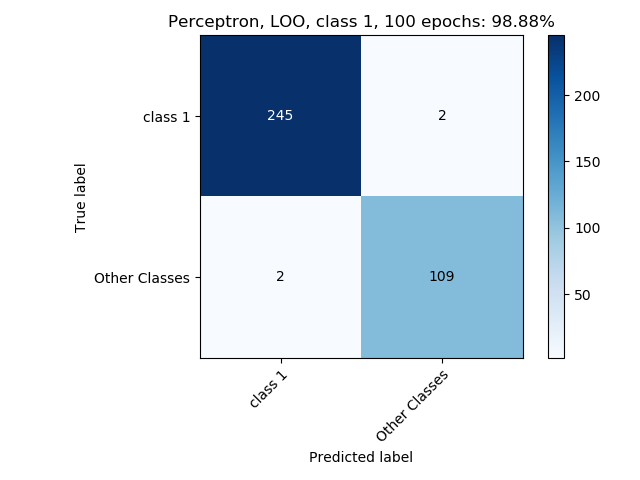
\includegraphics[width=\linewidth]{img/q3_fig_loo_classe1.png}
			\caption{Matriz de confusão para a classe 1}
			\label{fig:q1grau2}
		\end{subfigure}%
		\begin{subfigure}{.5\textwidth}
			\centering
			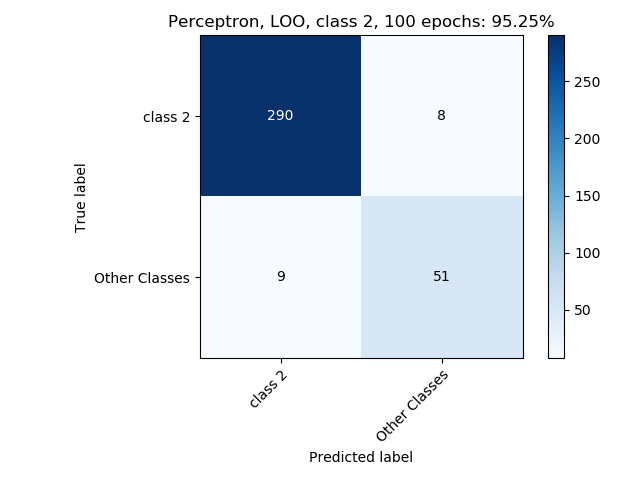
\includegraphics[width=\linewidth]{img/q3_fig_loo_classe2.png}
			\caption{Matriz de confusão para a classe 2}
			\label{fig:q1_grau3}
		\end{subfigure}
		\begin{subfigure}{.5\textwidth}
			\centering
			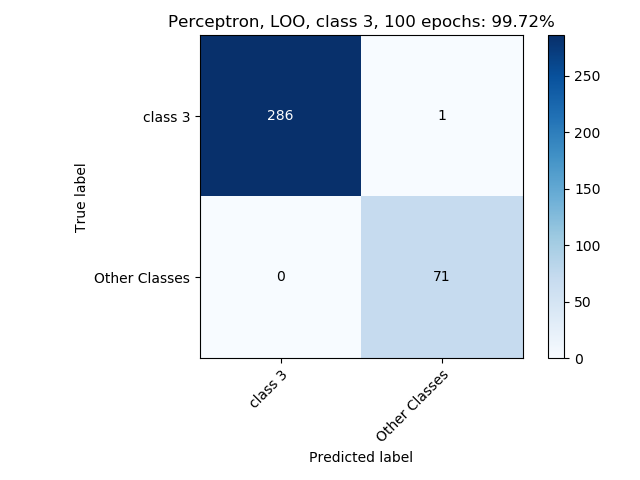
\includegraphics[width=\linewidth]{img/q3_fig_loo_classe3.png}
			\caption{Matriz de confusão para a classe 3}
			\label{fig:q1grau4}
		\end{subfigure}%
		\begin{subfigure}{.5\textwidth}
			\centering
			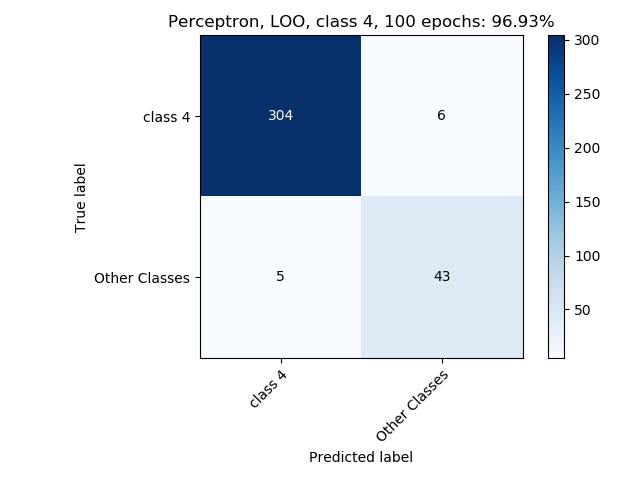
\includegraphics[width=\linewidth]{img/q3_fig_loo_classe4.png}
			\caption{Matriz de confusão para a classe 4}
			\label{fig:q1_grau5}
		\end{subfigure}
		\begin{subfigure}{.5\textwidth}
			\centering
			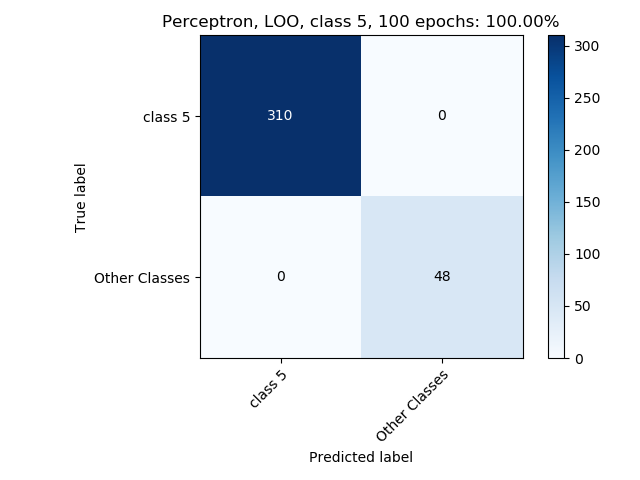
\includegraphics[width=\linewidth]{img/q3_fig_loo_classe5.png}
			\caption{Matriz de confusão para a classe 5}
			\label{fig:q1grau6}
		\end{subfigure}%
		\begin{subfigure}{.5\textwidth}
			\centering
			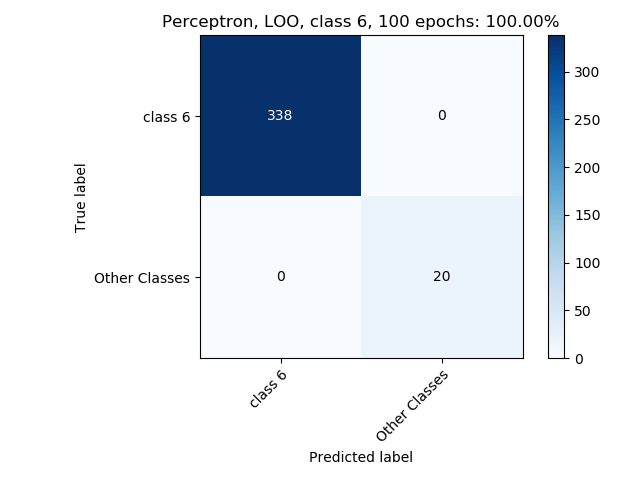
\includegraphics[width=\linewidth]{img/q3_fig_loo_classe6.png}
			\caption{Matriz de confusão para a classe 6}
			\label{fig:q1grau6}
		\end{subfigure}%
		
		\caption{Matrizes de confusão por classe utilizando \textit{Leave-one-out}}
		\label{fig:confusao_loo}
	\end{figure}
	
	\newpage
	.
	\newpage
% 	In the field of machine learning and specifically the problem of statistical classification, a confusion matrix, also known as an error matrix,[4] is a specific table layout that allows visualization of the performance of an algorithm, typically a supervised learning one (in unsupervised learning it is usually called a matching matrix). Each row of the matrix represents the instances in a predicted class while each column represents the instances in an actual class (or vice versa).[2] The name stems from the fact that it makes it easy to see if the system is confusing two classes (i.e. commonly mislabeling one as another).
	\subsubsection{'5-fold' (K-fold) }
	
	Assim como na subseção anterior, por estarmos utilizando uma rede perceptron, a classificação é feita individualmente para cada classe.
	
	Abaixo estão os resultados variando a quantidade de épocas para cada classe (sem normalização):
	
	\begin{multicols}{2}
    	\begin{verbatim}
For 1 epochs:
for class:1 Result:54.19 %
for class:2 Result:69.83 %
for class:3 Result:63.97 %
for class:4 Result:72.07 %
for class:5 Result:72.07 %
for class:6 Result:85.47 %
----------------------------
For 11 epochs:
for class:1 Result:84.36 %
for class:2 Result:77.93 %
for class:3 Result:97.49 %
for class:4 Result:66.48 %
for class:5 Result:92.74 %
for class:6 Result:97.21 %
----------------------------
For 21 epochs:
for class:1 Result:86.87 %
for class:2 Result:79.33 %
for class:3 Result:100.00 %
for class:4 Result:83.24 %
for class:5 Result:95.81 %
for class:6 Result:98.04 %
----------------------------
For 31 epochs:
for class:1 Result:95.81 %
for class:2 Result:74.30 %
for class:3 Result:100.00 %
for class:4 Result:82.12 %
for class:5 Result:98.60 %
for class:6 Result:98.60 %
----------------------------
For 41 epochs:
for class:1 Result:96.93 %
for class:2 Result:86.03 %
for class:3 Result:100.00 %
for class:4 Result:89.94 %
for class:5 Result:97.21 %
for class:6 Result:98.88 %
----------------------------
For 51 epochs:
for class:1 Result:96.65 %
for class:2 Result:85.75 %
for class:3 Result:100.00 %
for class:4 Result:81.28 %
for class:5 Result:98.60 %
for class:6 Result:98.88 %

    	\end{verbatim}
    \end{multicols}
    
    Abaixo estão os resultados variando a quantidade de épocas para cada classe (com normalização):
	
	\begin{multicols}{2}
    	\begin{verbatim}
For 1 epochs:
for class:1 Result:98.60 %
for class:2 Result:89.94 %
for class:3 Result:99.72 %
for class:4 Result:83.24 %
for class:5 Result:90.78 %
for class:6 Result:89.39 %
For 11 epochs:
for class:1 Result:99.16 %
for class:2 Result:98.88 %
for class:3 Result:100.00 %
for class:4 Result:99.72 %
for class:5 Result:100.00 %
for class:6 Result:99.72 %
----------------------------
For 21 epochs:
for class:1 Result:98.88 %
for class:2 Result:98.88 %
for class:3 Result:100.00 %
for class:4 Result:99.16 %
for class:5 Result:100.00 %
for class:6 Result:99.72 %
----------------------------
For 31 epochs:
for class:1 Result:98.88 %
for class:2 Result:100.00 %
for class:3 Result:100.00 %
for class:4 Result:99.44 %
for class:5 Result:100.00 %
for class:6 Result:99.72 %
----------------------------
For 41 epochs:
for class:1 Result:98.88 %
for class:2 Result:100.00 %
for class:3 Result:100.00 %
for class:4 Result:99.72 %
for class:5 Result:100.00 %
for class:6 Result:99.72 %
----------------------------
For 51 epochs:
for class:1 Result:98.88 %
for class:2 Result:100.00 %
for class:3 Result:100.00 %
for class:4 Result:99.72 %
for class:5 Result:100.00 %
for class:6 Result:99.72 %
----------------------------
    	\end{verbatim}
    \end{multicols}

    Outra forma de observar o desempenho da rede é através da matriz de confusão. A matriz de confusão é uma matriz quadrada de lado igual ao número de classes, e o valor de cada célula é a quantidade de vezes que a classe real foi igual a classe estimada.
	
	Na figura \ref{fig:confusao_loo} temos as matrizes de confusão para 100 épocas para cada classe.
	
	\begin{figure}[h!]
		\begin{subfigure}{.5\textwidth}
			\centering
			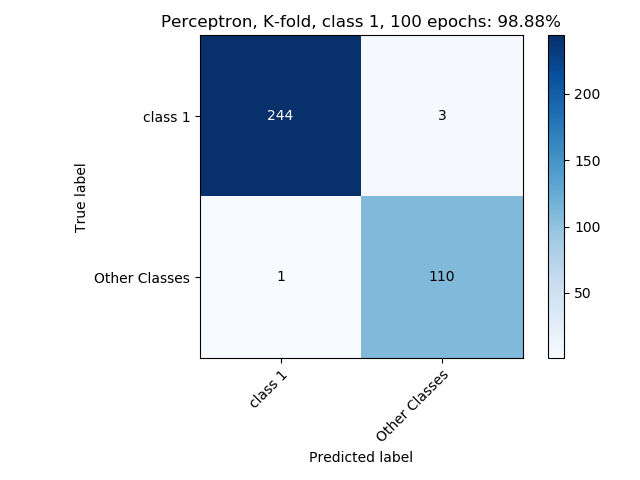
\includegraphics[width=\linewidth]{img/q3_fig_kfold_classe1.png}
			\caption{Matriz de confusão para a classe 1}
			\label{fig:q1grau2}
		\end{subfigure}%
		\begin{subfigure}{.5\textwidth}
			\centering
			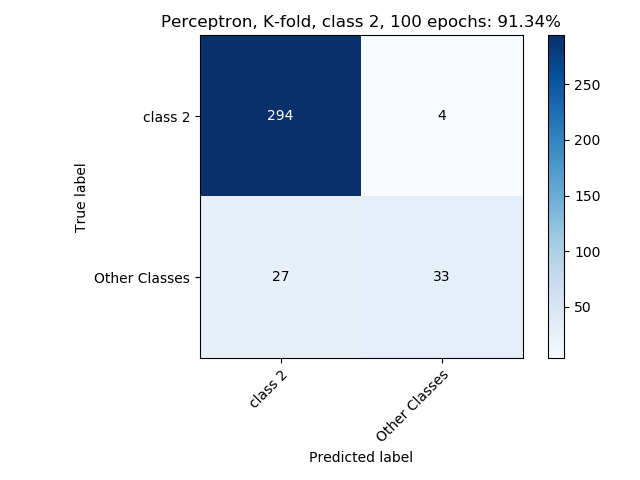
\includegraphics[width=\linewidth]{img/q3_fig_kfold_classe2.png}
			\caption{Matriz de confusão para a classe 2}
			\label{fig:q1_grau3}
		\end{subfigure}
		\begin{subfigure}{.5\textwidth}
			\centering
			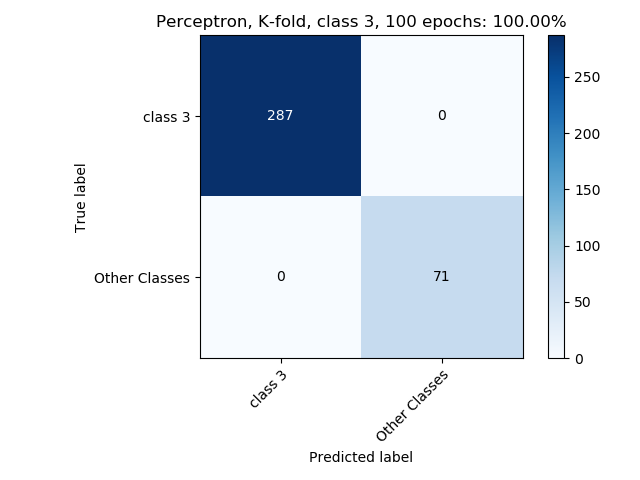
\includegraphics[width=\linewidth]{img/q3_fig_kfold_classe3.png}
			\caption{Matriz de confusão para a classe 3}
			\label{fig:q1grau4}
		\end{subfigure}%
		\begin{subfigure}{.5\textwidth}
			\centering
			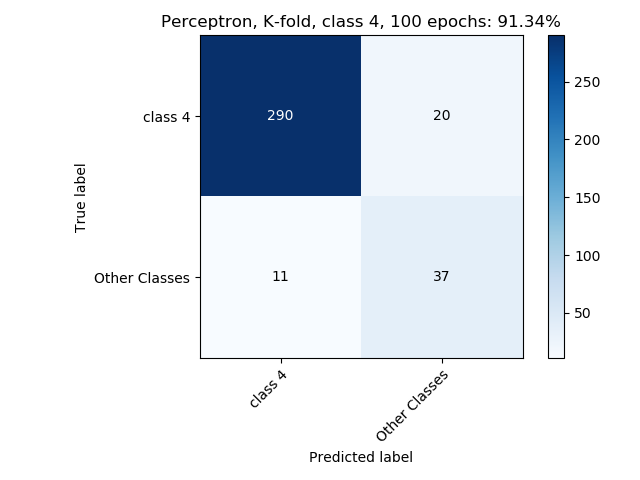
\includegraphics[width=\linewidth]{img/q3_fig_kfold_classe4.png}
			\caption{Matriz de confusão para a classe 4}
			\label{fig:q1_grau5}
		\end{subfigure}
		\begin{subfigure}{.5\textwidth}
			\centering
			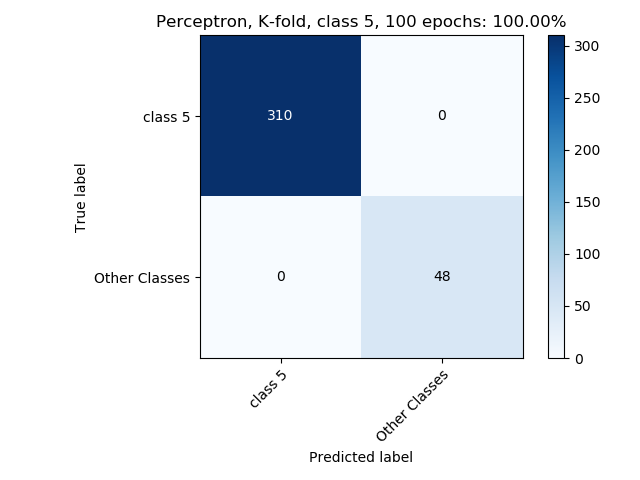
\includegraphics[width=\linewidth]{img/q3_fig_kfold_classe5.png}
			\caption{Matriz de confusão para a classe 5}
			\label{fig:q1grau6}
		\end{subfigure}%
		\begin{subfigure}{.5\textwidth}
			\centering
			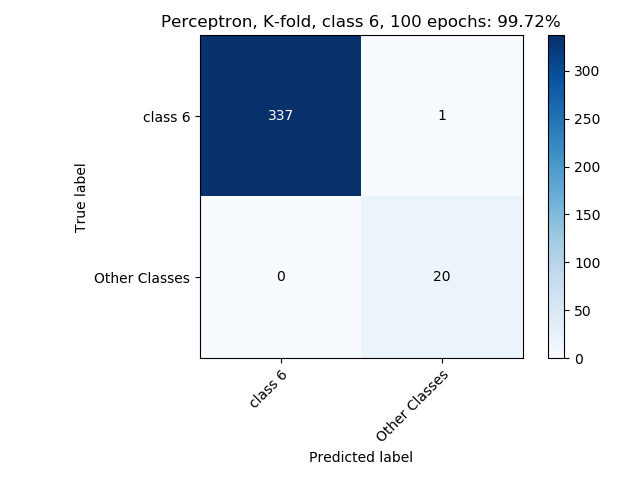
\includegraphics[width=\linewidth]{img/q3_fig_kfold_classe6.png}
			\caption{Matriz de confusão para a classe 6}
			\label{fig:q1grau6}
		\end{subfigure}%
		
		\caption{Matrizes de confusão por classe utilizando \textit{k-fold}}
		\label{fig:confusao_kfold}
	\end{figure}
	
	\newpage
	.
	\newpage
    
	\subsection{\textbf{Extreme Learning Machine}}
	
	Nessa subseção iremos mostrar os resultados utilizando ELM. Para o desenvolvimento do código do ELM foram utilizados apenas os slides dados em sala de aula como referência. Sua implementação é bastante direta e a fase de treinamento não funciona de forma iterativa. Na rede ELM há apenas uma camada oculta, que é inicializada com neuronios aleatorios.
    
    \subsubsection{K-fold}
    
	Podemos observar na Figura \ref{fig:ELM_confusao_kfold} que para a ELM é importante que os dados estejam normalizados. O desempenho da rede caiu em mais de 50\% para os dados não normalizados, tendo seu melhor resultado acertando 81.84\% e o pior desempenho acertando apenas 25.42\%.
    
	\begin{figure}[h!]
		\begin{subfigure}{.45\textwidth}
			\centering
			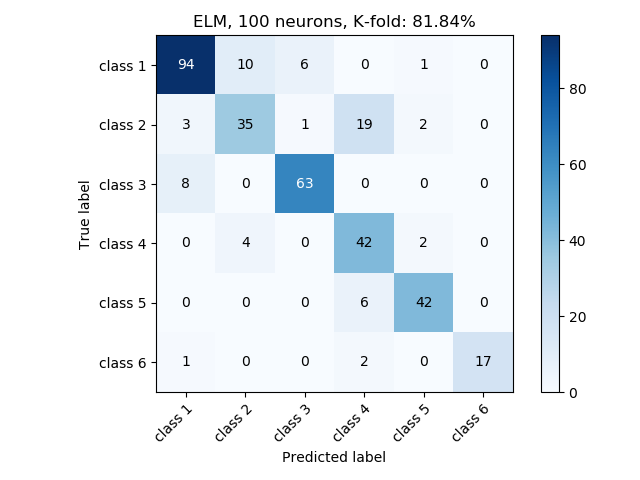
\includegraphics[width=\linewidth]{img/q3_elm_kfold_norm.png}
			\caption{Matriz de confusão com entrada normalizada}
			\label{fig:q1grau2}
		\end{subfigure}%
		\begin{subfigure}{.45\textwidth}
			\centering
			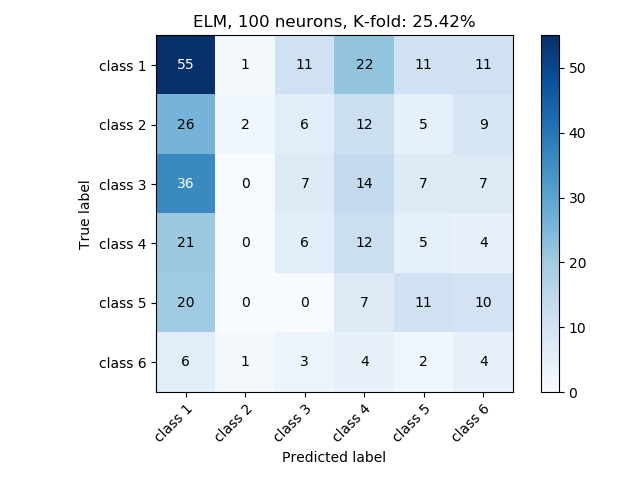
\includegraphics[width=\linewidth]{img/q3_elm_kfold_notNorm.png}
			\caption{Matriz de confusão com entrada não normalizada}
			\label{fig:q1_grau3}
		\end{subfigure}
		\caption{Matrizes de confusão utilizando \textit{k-fold}}
		\label{fig:ELM_confusao_kfold}
	\end{figure}
	

	\subsubsection{Leave-one-out}
	
	Utilizando leave-one-out também é possível observar (Figura \ref{fig:ELM_confusao_LOO}) que a normalização dos dados gera resultados bem mais significativos em relação aos dados não normalizados. Aqui o melhor resultado foi 83.52\%, marginalmente melhor que utilizando k-fold como validação. O pior resultado ficou com uma acurácia de 24.86\%, mostrando desempenho pior que a validação cruzada anterior.
	
	\begin{figure}[h!]
		\begin{subfigure}{.45\textwidth}
			\centering
			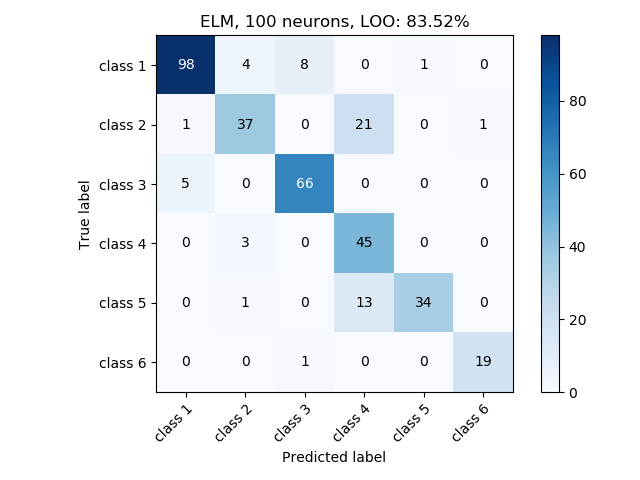
\includegraphics[width=\linewidth]{img/q3_elm_loo_norm.png}
			\caption{Matriz de confusão com entrada normalizada}
			\label{fig:q3mlpnorm}
		\end{subfigure}%
		\begin{subfigure}{.45\textwidth}
			\centering
			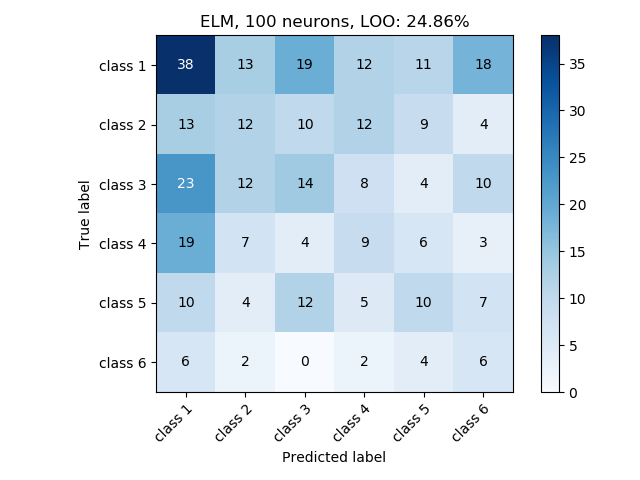
\includegraphics[width=\linewidth]{img/q3_elm_loo_notNorm.png}
			\caption{Matriz de confusão com entrada não normalizada}
			\label{fig:q3mlpnotnorm}
		\end{subfigure}
		\caption{Matrizes de confusão utilizando \textit{k-fold}}
		\label{fig:ELM_confusao_LOO}
	\end{figure}
	
	\newpage
	
	\subsection{\textbf{Multi-Layer Perceptron}}
	Nessa para os item utilizando MLP não foi necessário implementar a rede, por essa razão utilizei a biblioteca \textit{scikit-learn - Machine Learning in Python} para aplicar MLP no banco de dados.
	
	
	\subsubsection{K-fold}
	
	A rede MLP obteve os melhores resultados em relação a normalização dos dados. É possível observar que essa rede é mais resistente a dados não normalizados. Apesar de uma pequena perda de desempenho em dados não normalizados, foi possível uma acurácia de 95.81\% no melhor caso. Já nos dados não normalizados a acurácia caiu para 94.41\%.
	
	\begin{figure}[h!]
		\begin{subfigure}{.5\textwidth}
			\centering
			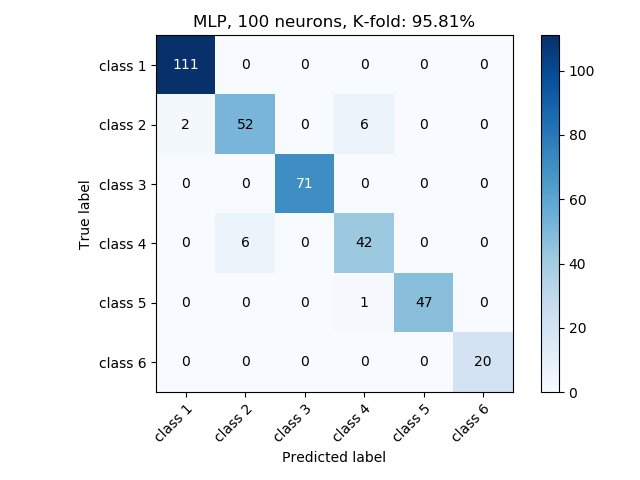
\includegraphics[width=\linewidth]{img/q3_mlp_kfold_norm.png}
			\caption{Matriz de confusão com entrada normalizada}
			\label{fig:q3loonorm}
		\end{subfigure}%
		\begin{subfigure}{.5\textwidth}
			\centering
			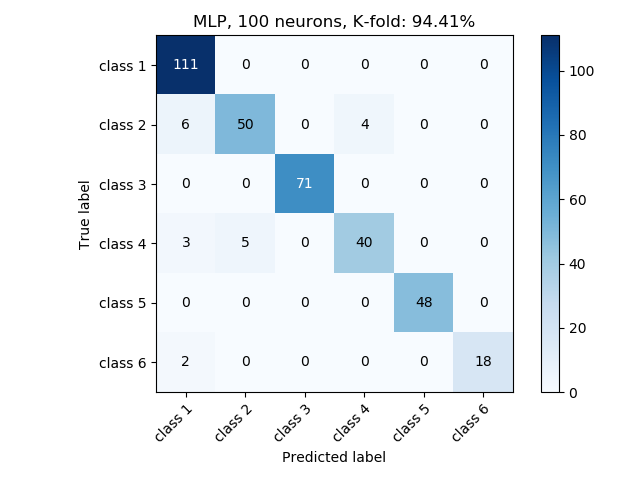
\includegraphics[width=\linewidth]{img/q3_mlp_kfold_notNorm.png}
			\caption{Matriz de confusão com entrada não normalizada}
			\label{fig:q3loonotnorm}
		\end{subfigure}
		\caption{Matrizes de confusão utilizando \textit{k-fold}}
		\label{fig:MLP_confusao_kfold}
	\end{figure}
	
	\subsubsection{Leave-one-out}
	
	Similar ao método de validação cruzada acima, a MLP também obteve bons resultados em relação a normalização dos dados.
    Seu desempenho ficou em 96.37\% para os dados normalizados e 94.97\% para o caso não normalizado.
	\begin{figure}[h!]
		\begin{subfigure}{.5\textwidth}
			\centering
			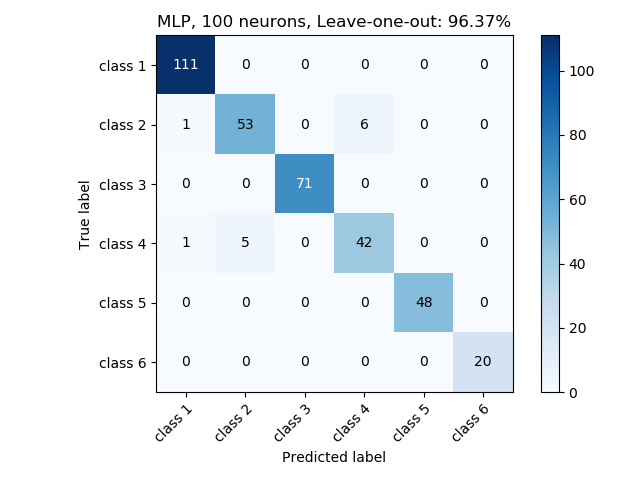
\includegraphics[width=\linewidth]{img/q3_mlp_loo_norm.png}
			\caption{Matriz de confusão com entrada normalizada}
			\label{fig:q3loonorm}
		\end{subfigure}%
		\begin{subfigure}{.5\textwidth}
			\centering
			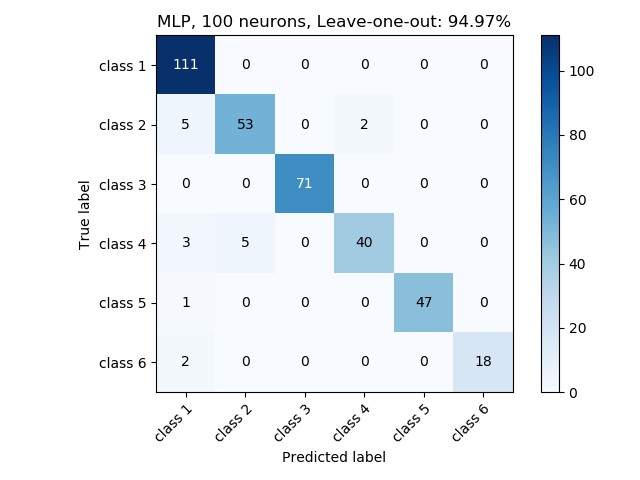
\includegraphics[width=\linewidth]{img/q3_mlp_loo_notNorm.png}
			\caption{Matriz de confusão com entrada não normalizada}
			\label{fig:q3loonotnorm}
		\end{subfigure}
		\caption{Matrizes de confusão utilizando \textit{k-fold}}
		\label{fig:MLP_confusao_LOO}
	\end{figure}
	
	\section{Código}
	
	Nessa seção será apresentada informações sobre como foram feitos os algoritmos e também os resultados desses algoritmos aplicados nas bases de dados para cada questão.
	
	\subsection{Programação}
	
	A linguagem de programação utilizada para resolver o problema foi \textit{Python 3.7}. Foram utilizadas as bibliotecas \textit{sklearn} e \textit{numpy} para auxiliar na aplicação das técnicas discutidas na seções 1 2 e 3, e também no tratamento de dados. 
	
	A base de dados “aerogerador.dat” contém 2250 amostras mapeando uma velocidade de vento para uma produção de energia.. Cada amostra da base contém apenas uma entrada e uma saída.
	
	A base de dados "Dermatology.dat" contém 358 amostras divididas em 6 classes. Cada amostra contém 34 \textit{features}.
    
	\section{Conclusão}
	
	Nesse relatório foram utilizados diferentes métodos de classificação, que foram testados utilizando 2 métodos de validação cruzada. As técnicas de classificação foram: MLP, ELM e perceptron.
	Existe um compromisso entre as diferentes técnicas, onde para bancos de dados diferentes pode haver técnicas de classificação mais adequadas.
	
	A normalização dos dados se mostrou bastante eficiente para algumas questões, levanta a taxa de acerto a valores mais de 50\% melhores. Porém na MLP sua influencia no resultado se mostrou bem menos efetiva..
	
	Todo o código desenvolvido para esse trabalho pode ser encontrado em \url{https://github.com/faellacurcio/rp} .
	
	\section{Apêndice}
	
	\subsection{Validação cruzada}
	Validação cruzada é uma de várias técnicas que é utilizada para estimar a qualidade de generalização de um algoritmo a partir da separação de um conjunto de dados. Seu principal objetivo é quantificar a eficiência de um modelo para a chegada de novos dados além de permitir a detecção de problemas como \textit{overfitting} (uma especialização excessiva no conjunto de dados perdendo assim a capacidade de generalização do modelo) . Em um modelo preditivo é típico haver dois grupos de dados: Dados de treinamento, dados de teste. Há diversas técnicas comumente utilizadas para realizar a validação cruzada.
	
	Validação cruzada é composta pela decomposição de um conjunto de dados em subconjuntos de treinamento e teste, podendo também incluir subconjunto de validação. O primeiro subconjunto, de treinamento, será utilizado para alimentar o modelo. Já o subconjunto, de teste, será utilizado para avaliar a porcentagem de acerto do modelo comparado a classificação do modelo com a classificação real. O ultimo conjunto, de validação, é utilizado em alguns classificadores como referencia para detectar \textit{overfitting} como é feito em redes neurais. Uma regra de ouro da validação cruzada diz que os conjuntos de treinamento, teste e validação não devem possuir elementos em comum! As sub-sessões abaixo exemplificam os métodos de validação cruzada utilizadas no trabalho de Reconhecimento de padrões.
	
	\subsection{\textit{Leave-one-out}}
	Esse método de é um dos mais simples de ser implementado. Ele consistem em utilizar o conjunto completo menos uma amostra para o subconjunto de treinamento, e apenas essa amostra que não foi incluída no grupo de treinamento para ser o subconjunto teste. Para um conjunto de N pontos, são utilizados N-1 amostas no subconjuntos de treinamento e 1 amostra no subconjunto de teste como é mostrado na Figura \ref{fig:loo}. A eficiência do modelo é dada em porcentagem pela média de acertos. 
	
	\begin{figure}[h!]
		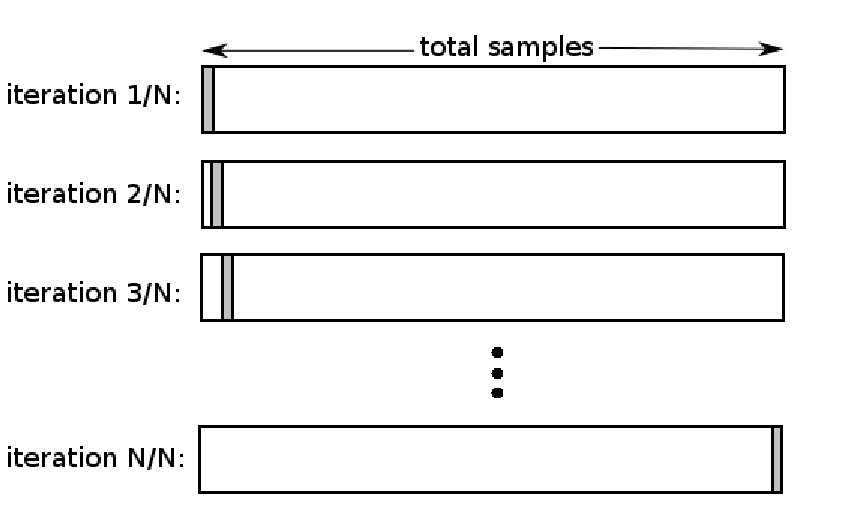
\includegraphics[width=8cm]{img/Leave-One-Out-Cross-Validation.png}
		\centering
		\caption{Validação cruzada \textit{leave-one-out}}
		\label{fig:loo}
	\end{figure}
	
	\subsection{\textit{k-fold}}
	
	O \textit{k-fold} pode ser visto como uma extensão do \textit{leave-one-out} porém ao invés de utilizar uma única amostra para o conjunto de teste, os dados serão divididos em K conjuntos de aproximadamente mesmo tamanho. Similarmente ao que foi mostrado na sub-seção anterior, esse método é utilizado para estimar o quão eficaz o modelo será ao encontrar dados novos, ou seja, quantificar a eficiência de uma técnica de classificação. A figura \ref{fig:kfold} mostra a divisão dos dados, onde cada bloco (\textit{train/test}) contém \textbf{k} conjuntos de aproximadamente mesmo tamanho.
	
	\begin{figure}[h!]
		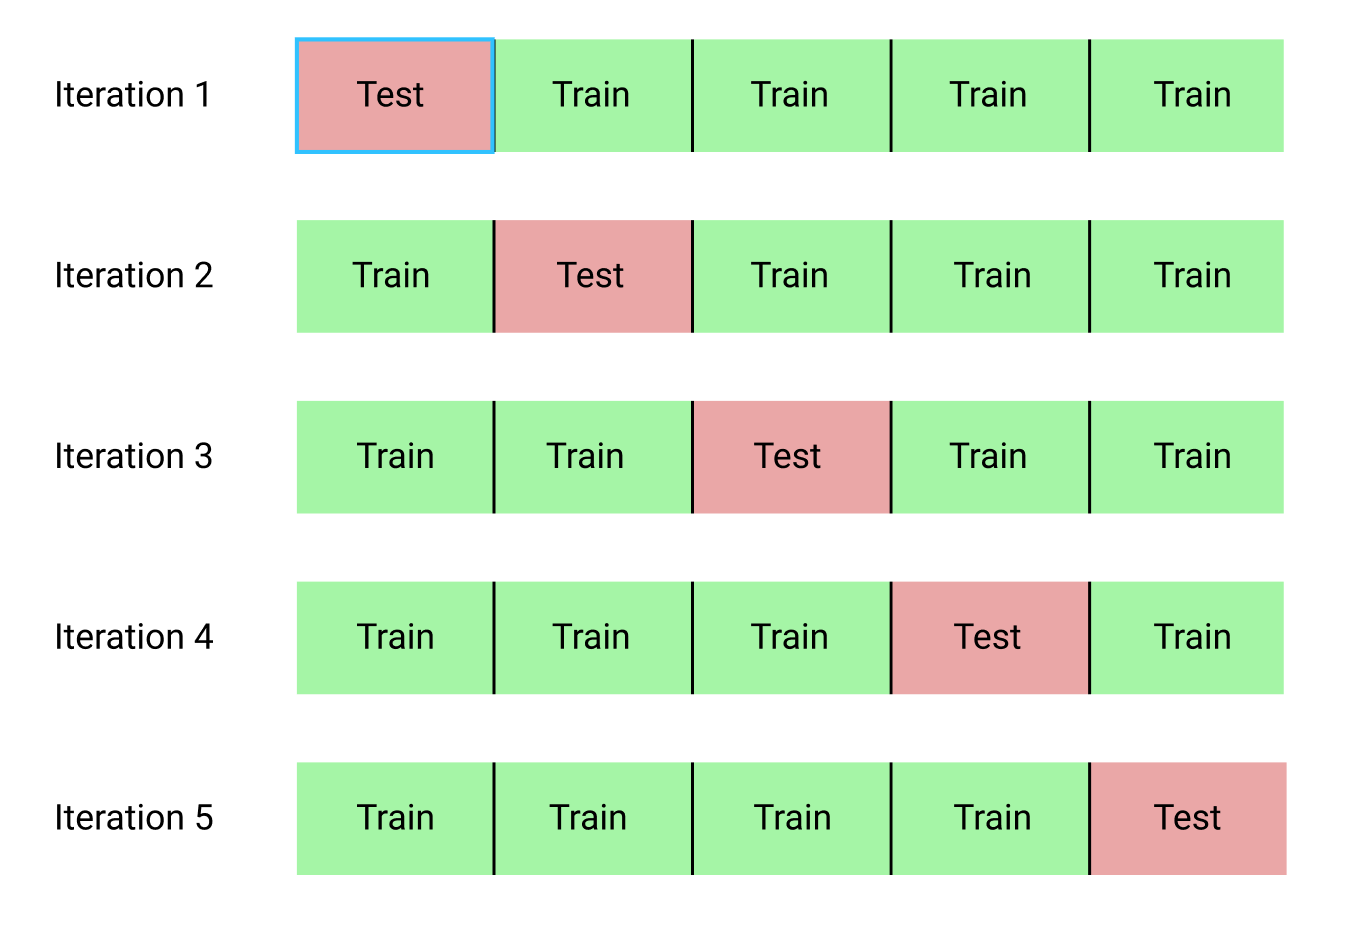
\includegraphics[width=7cm]{img/k-fold1.png}
		\centering
		\caption{Validação cruzada \textit{k-fold}}
		\label{fig:kfold}
	\end{figure}
	
	
% 	\begin{figure}[h]
% 		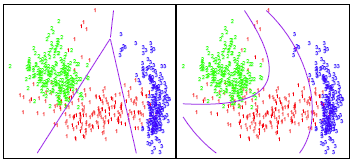
\includegraphics[width=8cm]{img/LDAQDA.png}
% 		\centering
% 		\caption{Diferentes curvas de decisão geradas em LDA e QDA}
% 		\label{fig:ldaqda}
% 	\end{figure}
	
	
	%%% End document
\end{document}


% KFOLD
% For 1 epochs:
% for class:1 Result:54.19 %
% for class:2 Result:69.83 %
% for class:3 Result:63.97 %
% for class:4 Result:72.07 %
% for class:5 Result:72.07 %
% for class:6 Result:85.47 %
% For 11 epochs:
% for class:1 Result:84.36 %
% for class:2 Result:77.93 %
% for class:3 Result:97.49 %
% for class:4 Result:66.48 %
% for class:5 Result:92.74 %
% for class:6 Result:97.21 %
% For 21 epochs:
% for class:1 Result:86.87 %
% for class:2 Result:79.33 %
% for class:3 Result:100.00 %
% for class:4 Result:83.24 %
% for class:5 Result:95.81 %
% for class:6 Result:98.04 %
% For 31 epochs:
% for class:1 Result:95.81 %
% for class:2 Result:74.30 %
% for class:3 Result:100.00 %
% for class:4 Result:82.12 %
% for class:5 Result:98.60 %
% for class:6 Result:98.60 %
% For 41 epochs:
% for class:1 Result:96.93 %
% for class:2 Result:86.03 %
% for class:3 Result:100.00 %
% for class:4 Result:89.94 %
% for class:5 Result:97.21 %
% for class:6 Result:98.88 %
% For 51 epochs:
% for class:1 Result:96.65 %
% for class:2 Result:85.75 %
% for class:3 Result:100.00 %
% for class:4 Result:81.28 %
% for class:5 Result:98.60 %
% for class:6 Result:98.88 %
% For 61 epochs:
% for class:1 Result:98.88 %
% for class:2 Result:81.28 %
% for class:3 Result:100.00 %
% for class:4 Result:88.55 %
% for class:5 Result:98.60 %
% for class:6 Result:99.44 %
% For 71 epochs:
% for class:1 Result:98.88 %
% for class:2 Result:85.75 %
% for class:3 Result:100.00 %
% for class:4 Result:88.55 %
% for class:5 Result:100.00 %
% for class:6 Result:99.44 %
% For 81 epochs:
% for class:1 Result:98.88 %
% for class:2 Result:84.64 %
% for class:3 Result:100.00 %
% for class:4 Result:88.27 %
% for class:5 Result:100.00 %
% for class:6 Result:99.72 %
% For 91 epochs:
% for class:1 Result:98.88 %
% for class:2 Result:91.06 %
% for class:3 Result:100.00 %
% for class:4 Result:90.78 %
% for class:5 Result:100.00 %
% for class:6 Result:99.72 %N

% Leave one out
% For 1 epochs:
% for class:1 Result:94.69 %
% for class:2 Result:84.08 %
% for class:3 Result:98.88 %
% for class:4 Result:86.31 %
% for class:5 Result:98.60 %
% for class:6 Result:98.32 %

% For 2 epochs:
% for class:1 Result:96.65 %
% for class:2 Result:80.73 %
% for class:3 Result:99.72 %
% for class:4 Result:89.39 %
% for class:5 Result:99.44 %
% for class:6 Result:99.16 %

% For 3 epochs:
% for class:1 Result:96.09 %
% for class:2 Result:90.78 %
% for class:3 Result:99.44 %
% for class:4 Result:92.74 %
% for class:5 Result:98.60 %
% for class:6 Result:100.00 %
% For 4 epochs:
% for class:1 Result:98.04 %
% for class:2 Result:92.46 %
% for class:3 Result:99.72 %
% for class:4 Result:94.69 %
% for class:5 Result:98.88 %
% for class:6 Result:100.00 %
% For 5 epochs:
% for class:1 Result:97.77 %
% for class:2 Result:90.78 %
% for class:3 Result:99.44 %
% for class:4 Result:94.41 %
% for class:5 Result:99.72 %
% for class:6 Result:100.00 %
% For 6 epochs:
% for class:1 Result:98.32 %
% for class:2 Result:93.85 %
% for class:3 Result:100.00 %
% for class:4 Result:94.13 %
% for class:5 Result:99.72 %
% for class:6 Result:100.00 %
% For 7 epochs:
% for class:1 Result:98.60 %
% for class:2 Result:93.58 %
% for class:3 Result:100.00 %
% for class:4 Result:94.97 %
% for class:5 Result:100.00 %
% for class:6 Result:100.00 %
% For 8 epochs:
% for class:1 Result:98.88 %
% for class:2 Result:94.41 %
% for class:3 Result:100.00 %
% for class:4 Result:95.25 %
% for class:5 Result:99.44 %
% for class:6 Result:100.00 %